\documentclass{standalone}

\usepackage{pgfplots}

\usetikzlibrary{angles, quotes, calc, intersections}

\pgfplotsset{compat=newest}

\begin{document}
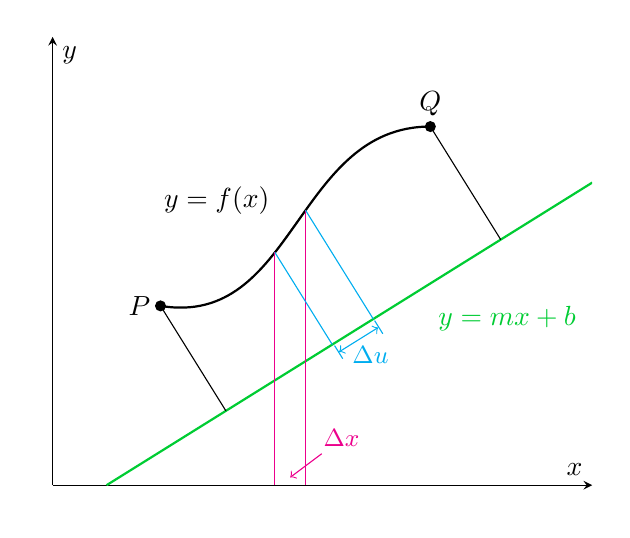
\begin{tikzpicture}
    \begin{axis}[axis lines=center, xlabel=$x$, ylabel=$y$, tick style={draw=none}, xticklabel=\empty, yticklabel=\empty, xmin=0, xmax=10, ymin=0, ymax=10]
        \pgfmathsetmacro{\Px}{2}
        \pgfmathsetmacro{\Py}{4}
        \pgfmathsetmacro{\Qx}{7}
        \pgfmathsetmacro{\Qy}{8}
        \pgfmathsetmacro{\m}{0.75}
        \pgfmathsetmacro{\b}{1}

        \pgfplotsextra{
        % endpoints of curve
        \coordinate (P) at (\Px, \Py);
        \coordinate (Q) at (\Qx, \Qy);

        % line
        \draw[thick, green!80!blue] (\b, 0) -- node[right, xshift=1cm, yshift=2mm] {$y = m x + b$} (10, {\m * (10 - \b)});

        % curve
        \draw[thick, black] (P) node[left] {$P$} .. controls ({(\Px + \Qx) / 2}, \Py - 0.5) and ({(\Px + \Qx) / 2}, \Qy) .. node[above, xshift=-1cm] {$y = f(x)$} (Q) node[above] {$Q$} coordinate[pos=0.4] (M) coordinate[pos=0.55] (N);

        % ordinals
        \draw (P) -- ($(0, {-\m * \b})!(P)!(\b, 0)$);
        \draw (Q) -- ($(0, {-\m * \b})!(Q)!(\b, 0)$);

        % dots
        \fill (P) circle (2pt);
        \fill (Q) circle (2pt);

        \coordinate (X1) at ($(0, 0)!(M)!(1, 0)$);
        \coordinate (X2) at ($(0, 0)!(N)!(1, 0)$);
        \coordinate (U1) at ($(0, {-\m * \b})!(M)!(\b, 0)$);
        \coordinate (U2) at ($(0, {-\m * \b})!(N)!(\b, 0)$);

        % partition lines
        \draw (M) -- (N);
        \draw[magenta] (M) -- (X1) (N) -- (X2);
        \draw[cyan] (U1) -- (M) (N) -- (U2);

        \draw[magenta, <-] ([yshift=1mm]$(X1)!0.5!(X2)$) -- ++(4mm, 3mm) node[right, xshift=-1mm, yshift=2mm] {\small$\Delta x$};
        \draw[cyan, |<->|] ([xshift=\m mm, yshift=-1 mm]U1) -- node[xshift=2*\m mm, yshift=-2mm] {\small$\Delta u$} ([xshift=\m mm, yshift=-1 mm]U2);
        }
    \end{axis}
\end{tikzpicture}
\end{document}
